\chapter{Listas e Tabelas}

Este capítulo aborda a importância de se utilizar listas e tabelas no HTML para exibir dados de forma clara e organizada. O HTML é uma linguagem de marcação que permite a criação de diferentes estruturas dentro de uma página web, e listas e tabelas são elementos fundamentais para apresentar dados de maneira estruturada e fácil de compreender.

Listas permitem apresentar informações em uma série de itens relacionados, sejam eles numerados ou marcados. Já as tabelas são usadas para exibir informações em forma de linhas e colunas, facilitando a comparação e a análise de dados.

Neste capítulo, você aprenderá sobre os diferentes tipos de listas e tabelas que podem ser criados com HTML, bem como as \textit{tags} e atributos necessários para sua implementação. Em resumo, ao final deste capítulo, você estará capacitado a criar listas e tabelas eficientes para suas páginas web, garantindo uma apresentação clara e organizada de dados.

\section{Listas}

Listas são elementos HTML que permitem organizar e apresentar informações de maneira estruturada e fácil de entender. Em HTML, existem três tipos principais de listas: listas não-ordenadas (\textit{unordered lists}), listas ordenadas (\textit{ordered lists}) e listas de definições (\textit{definition lists}). Listas não-ordenadas são usadas para apresentar informações em que a ordem dos itens não é importante, como uma lista de ingredientes ou de itens de um cardápio. Listas ordenadas são usadas para apresentar informações em que a ordem dos itens é importante, como uma lista de instruções de montagem de um móvel ou uma lista cronológica de tarefas a fazer. Listas de definições, por sua vez, são usadas para apresentar termos e suas respectivas descrições, como em um dicionário, onde temos uma palavra e seu significado.

O propósito de usar listas na web é o de exibir dados em uma página de maneira clara e fácil de entender para o usuário, em uma estrutura sequencial ordenada ou não ordenada. Além disso, listas são uma ótima maneira de tornar o conteúdo da página acessível para usuários com necessidades especiais, como os usuários de leitor de tela, pois eles podem navegar facilmente pelos itens da lista um a um. Agora veremos como usar cada um dos tipos de lista mencionados.

\subsection{Listas Não Ordenadas}

As listas não ordenadas são usadas para apresentar uma série de itens em que a ordem não é importante. Como exemplos de uso, podemos citar ingredientes de uma receita, especificações técnicas de um produto etc. Em HTML, essas listas são criadas usando o elemento \var{<ul>} (\textit{unordered lists}) e cada item da lista é criado usando o elemento \var{<li>} (\textit{list item}).

A lista não ordenada é apresentada com marcadores (bolinhas, quadrados etc.) antes de cada item da lista. O tipo de marcador pode ser alterado usando o atributo \var{type}. Por exemplo, o valor \var{square} apresenta quadrados como marcadores, \var{circle} apresenta um círculo e o valor \var{disc}, que é o padrão, apresenta bolinhas. O exemplo \ref{code:ul} mostra o código de uma lista não ordenada e a figura \ref{fig:ul} mostra a renderização do exemplo.

\begin{htmlcode}{Lista não ordenada básica.}{code:ul}
<ul>
    <li>Item 1</li>
    <li>Item 2</li>
    <li>Item 3</li>
</ul>
\end{htmlcode}

\begin{figure}[ht!]    
    \frame{
    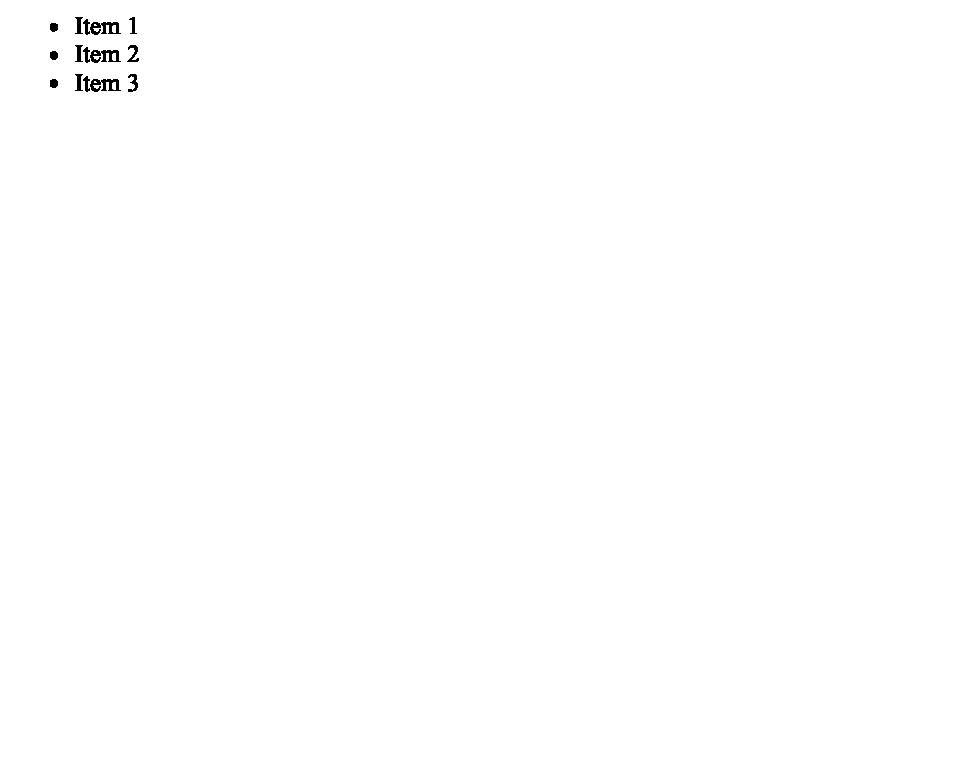
\includegraphics[width=.3\textwidth, trim={0 11.2cm 12cm 0}]{Images/chapter03/html_ul.pdf}}
    \caption{Renderização da lista não ordenada do exemplo \ref{code:ul}.}
    \label{fig:ul}
\end{figure}

Vamos agora ver um exemplo de lista não ordenada com marcadores quadrados. O código do exemplo \ref{code:ul_square} mostra uma lista não ordenada com marcadores quadrados, enquanto a figura \ref{fig:ul_square} mostra a renderização do código em questão. Veja na linha 1 do código que agora o atributo \var{type="square"\textgreater} está presente na \textit{tag} de abertura do elemento \var{<ul>}.

\begin{htmlcode}{Lista não ordenada com marcador quadrado.}{code:ul_square}
<ul type="square">
    <li>Item 1</li>
    <li>Item 2</li>
    <li>Item 3</li>
</ul>
\end{htmlcode}

\begin{figure}[ht!]    
    \frame{
    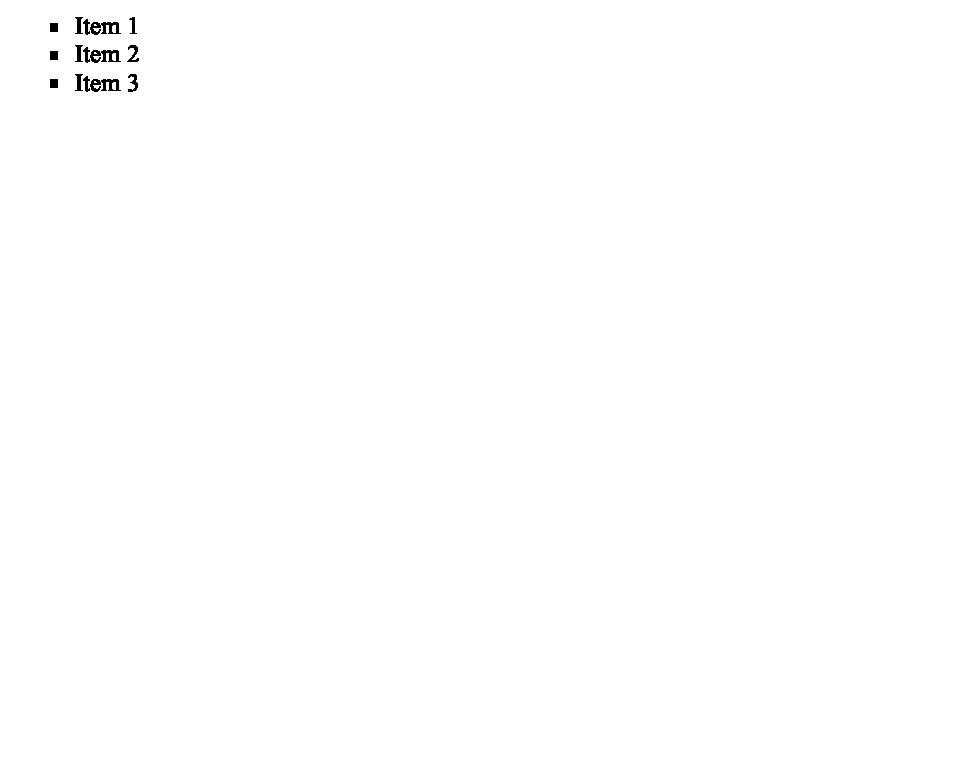
\includegraphics[width=.3\textwidth, trim={0 11.2cm 12cm 0}]{Images/chapter03/html_ul_square.pdf}}
    \caption{Renderização da lista não ordenada com marcador quadrado do exemplo \ref{code:ul_square}.}
    \label{fig:ul_square}
\end{figure}

\subsection{Listas Ordenadas}

As listas ordenadas são usadas para apresentar uma série de itens em que a ordem é importante. Em HTML, essas listas são criadas usando o elemento \var{<ol>} (\textit{ordered list}) e cada item da lista é criado usando o elemento \var{<li>} (\textit{list item}).

A lista ordenada é apresentada com números ou letras antes de cada item da lista, indicando a ordem dos itens. O tipo de número ou letra pode ser alterado usando o atributo \var{type}. Por exemplo, o valor \var{A} apresenta letras maiúsculas como marcadores, enquanto o valor "i" apresenta letras minúsculas romanas como marcadores. Se o atributo \var{type} não for passado, a lista é numerada com algarismos arábicos iniciando em 1. O exemplo \ref{code:ol} mostra o código de uma lista ordenada e a figura \ref{fig:ol} mostra a renderização do exemplo. Veja que os marcadores são algarismos romanos em maiúsculas.

\begin{htmlcode}{Lista ordenada com algarismos romanos.}{code:ol}
<ol type="I">
    <li>HTML</li>
    <li>CSS</li>
    <li>Javascript</li>
</ol>
\end{htmlcode}

\begin{figure}[ht!]    
    \frame{
    
\includegraphics[width=.3\textwidth, trim={0 11.2cm 12cm 0}]{Images/chapter03/html_ol.pdf}}
    \caption{Renderização da lista ordenada do exemplo \ref{code:ol}.}
    \label{fig:ol}
\end{figure}

Outros dois atributos podem ser usados em listas ordenadas. O atributo \var{start} permite que você informe um valor inicial para a numeração dos itens. Por exemplo, se você passar \var{start="5"}, o primeiro elemento da lista iniciará com o valor 5. O outro atributo é o \var{reversed}, que não possui valor. A presença do atributo \var{reversed} faz com que a lista seja exibida na ordem inversa.

Assim como ocorre com listas não ordenadas, as listas ordenadas também são uma ótima maneira de tornar o conteúdo da página acessível para usuários com necessidades especiais, como usuários de leitor de tela, pois permitem que esses usuários naveguem item por item.

\subsection{Listas de Definições}

As listas de definições são usadas para apresentar termos e descrições, como em um dicionário. Em HTML, essas listas são criadas usando os elementos \var{<dl>} (\textit{definition list}), \var{<dt>} (\textit{definition term}) e \var{<dd>} (\textit{definition description}). O elemento \var{<dt>} é usado para definir o termo, enquanto o elemento \var{<dd>} é usado para descrever o termo. Cada termo e sua descrição formam um par de definição. O exemplo \ref{code:dl} mostra o código de uma lista de definições e a figura \ref{fig:dl} mostra a renderização desse código.

\begin{htmlcode}{Lista de definições.}{code:dl}
<dl>
    <dt>HTML</dt>
    <dd>Linguagem de Marcação Hipertexto</dd>
    <dt>CSS</dt>
    <dd>Folha de Estilo em Cascata</dd>
    <dt>JavaScript</dt>
    <dd>Linguagem de Programação de Script</dd>
</dl>
\end{htmlcode}

\begin{figure}[ht!]    
    \frame{
    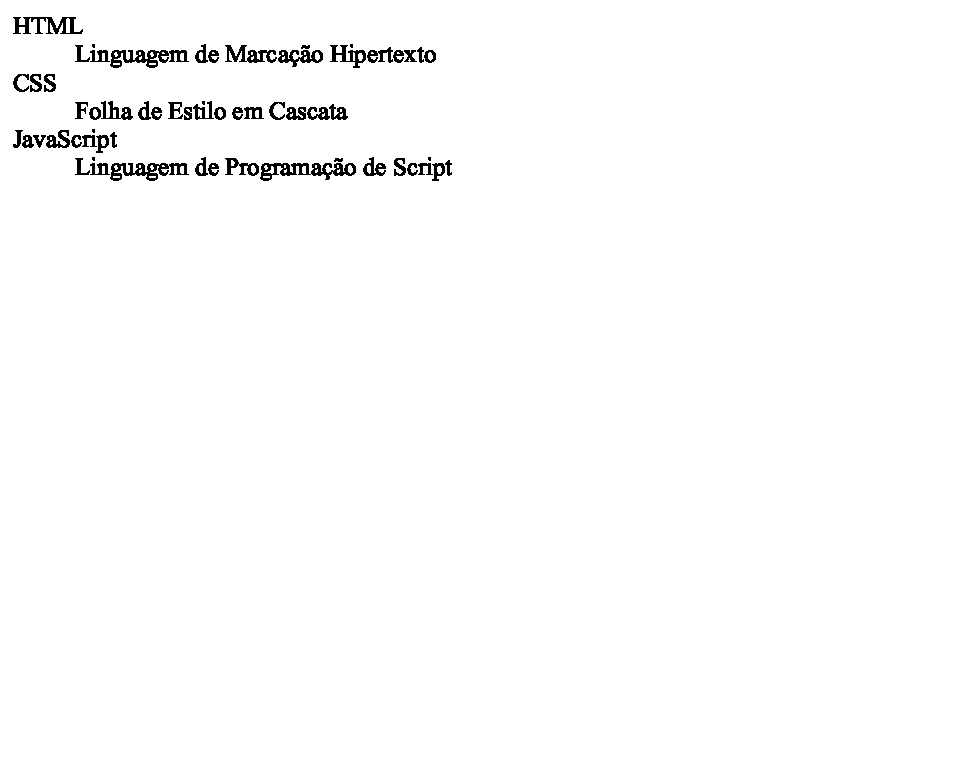
\includegraphics[width=.45\textwidth, trim={0 9.7cm 8cm 0}]{Images/chapter03/html_dl.pdf}}
    \caption{Renderização da lista de definições do exemplo \ref{code:dl}.}
    \label{fig:dl}
\end{figure}

As listas de definições são úteis para apresentar informações de maneira clara e fácil de entender para o usuário, especialmente quando se trata de definir ou descrever termos técnicos ou complexos. Além disso, elas também são uma ótima maneira de tornar o conteúdo da página acessível para usuários com necessidades especiais, como usuários de leitor de tela.

\section{Tabelas}

As tabelas são um recurso fundamental na construção de páginas web, pois permitem a organização de informações em linhas e colunas, facilitando a visualização e comparação de dados. Na HTML, as tabelas são criadas com a utilização de \textit{tags} específicas, permitindo que sejam criados diversos tipos de estruturas, como tabelas simples, tabelas com células mescladas, tabelas com cabeçalhos e rodapés, entre outras.

\subsection{Tabelas Simples}

As tabelas simples são o tipo mais comum de tabela HTML e consistem em uma grade retangular formada por \textbf{linhas} e \textbf{colunas}, em que cada \textbf{célula} pode conter texto, imagens ou outros elementos HTML. Elas são uma maneira eficiente de organizar e apresentar informações em formato tabular, facilitando a leitura e a compreensão de dados.

As tabelas simples podem ser utilizadas em diversas situações, como em listas de preços, horários, agenda de eventos, entre outros. Elas permitem que informações sejam apresentadas em colunas e linhas, com cabeçalhos e rodapés para cada seção, permitindo a comparação de dados e informações. O exemplo \ref{code:table} mostra o código de uma tabela simples com a primeira linha como cabeçalho.

\begin{htmlcode}{Tabela simples.}{code:table}
<table>
    <tr>
        <th>Produto</th>
        <th>Preço</th>
    </tr>
    <tr>
        <td>Camiseta</td>
        <td>R$ 39,90</td>
    </tr>
    <tr>
        <td>Calça Jeans</td>
        <td>R$ 89,90</td>
    </tr>
    <tr>
        <td>Tênis</td>
        <td>R$ 129,90</td>
    </tr>
</table>
\end{htmlcode}

Neste exemplo \ref{code:table}, temos uma tabela com duas colunas, uma para o nome do produto e outra para o preço. A primeira linha da tabela é o cabeçalho, e é definida com o elemento \var{<tr>} para a linha que, por sua vez, contém elementos \var{<th>} para os títulos das colunas. Observe que, por padrão, o conteúdo textual das células de título é exibido em negrito. As linhas de dados são definidas com o elemento \var{<tr>} e as células de dados com o elemento \var{<td>}. A figura \ref{fig:table} mostra como fica a renderização dessa tabela.

\begin{figure}[ht!]    
    \frame{
    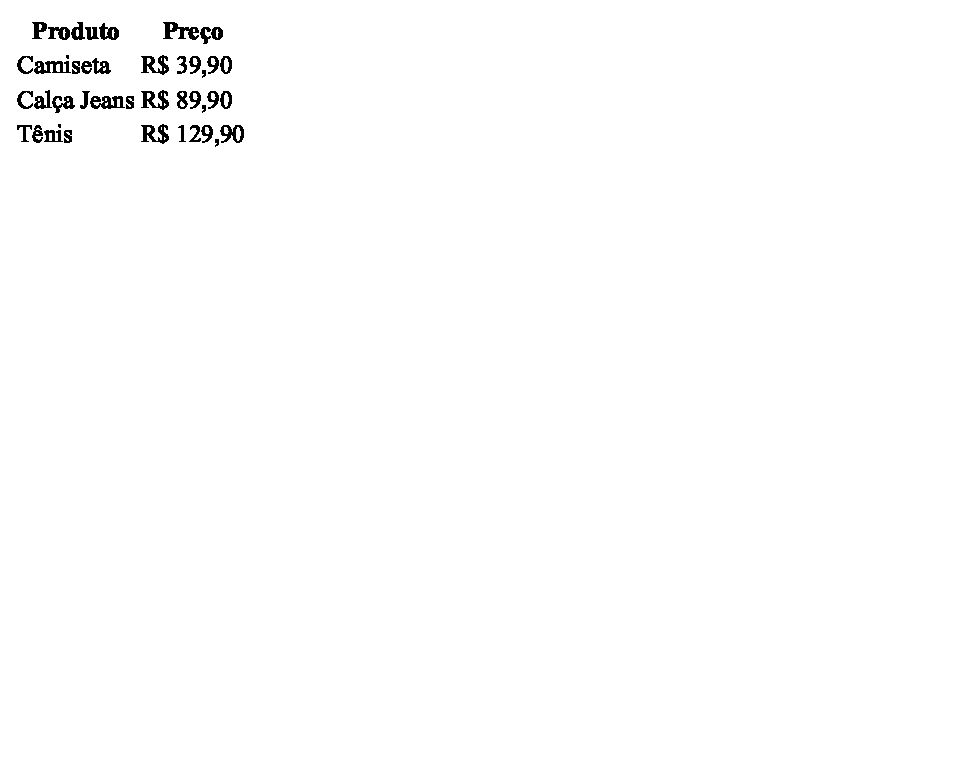
\includegraphics[width=.4\textwidth, trim={0 10cm 11cm 0}]{Images/chapter04/html_table.pdf}}
    \caption{Renderização da tabela do exemplo \ref{code:table}.}
    \label{fig:table}
\end{figure}

Apenas com a finalidade de melhorar a visualização das divisões entre as células das tabelas ao longo deste material, eu vou usar o atributo \var{border} com o valor igual a \var{1} para que bordas sejam adicionadas à tabela e às suas células. Esse atributo está obsoleto, portanto, seu uso não é recomendado, uma vez que pode-se obter resultados melhores usando CSS, como veremos na parte II deste material. Enquanto não aprendemos a fazer bordas com CSS, vamos usar o atributo \var{border}. O exemplo \ref{code:table_border} mostra o código de uma tabela com o atributo \var{border} e a figura \ref{fig:table_border} mostra sua renderização.

\begin{htmlcode}{Tabela com bordas.}{code:table_border}
<table border="1">
    <tr>
        <th>Nome</th>
        <th>Idade</th>
    </tr>
    <tr>
        <td>João</td>
        <td>30</td>
    </tr>
    <tr>
        <td>Maria</td>
        <td>25</td>
    </tr>
</table>
\end{htmlcode}

\begin{figure}[ht!]    
    \frame{
    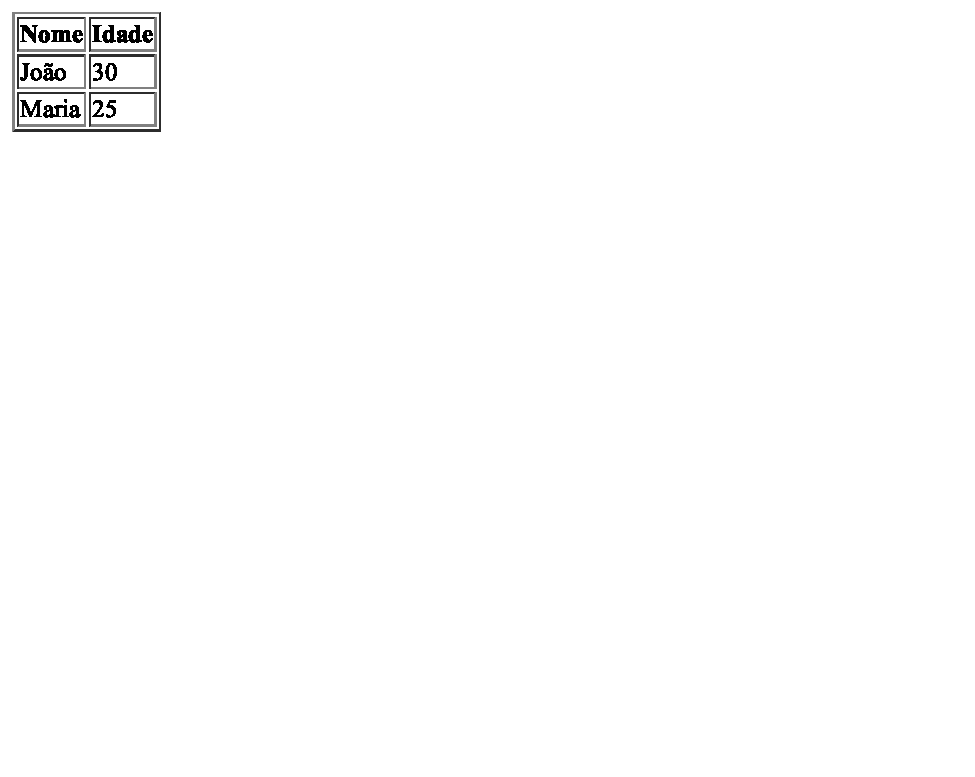
\includegraphics[width=.25\textwidth, trim={0 10.5cm 13cm 0}]{Images/chapter04/html_table_border.pdf}}
    \caption{Renderização da tabela do exemplo \ref{code:table_border}.}
    \label{fig:table_border}
\end{figure}

\subsection{Cabeçalho, Corpo e Rodapé}

Os elementos \var{<thead>}, \var{<tbody>} e \var{<tfoot>} são usados para separar diferentes partes de uma tabela HTML. Eles são opcionais, mas podem ajudar a organizar e estruturar melhor o conteúdo e aprimoram o aspecto semântico da tabela.

O elemento \var{<thead>} é usado para definir o cabeçalho da tabela. Ele deve ser usado apenas uma vez e deve ser colocado no início da tabela. O \var{<thead>} pode conter uma ou mais linhas (\var{<tr>}) e as células (\var{<th>}) representam os cabeçalhos das colunas. Ao utilizar o elemento \var{<thead>}, as células de cabeçalho podem ser diferenciadas visualmente do conteúdo da tabela, melhorando a legibilidade.

O elemento \var{<tbody>} é usado para agrupar o conteúdo da tabela em um ou mais blocos. Ele pode ser usado várias vezes dentro da tabela, mas deve ser colocado após o elemento \var{<thead>}, se este estiver presente. O \var{<tbody>} contém uma ou mais linhas (\var{<tr>}) e as células (\var{<td>}) representam os dados de cada coluna. Quando há várias linhas, é possível estilizar a tabela para diferenciar visualmente cada bloco de dados.

Por fim, o elemento \var{<tfoot>} é usado para definir o rodapé da tabela. Ele também deve ser usado apenas uma vez e deve ser colocado no final da tabela, após o último \var{<tbody>}. O \var{<tfoot>} pode conter uma ou mais linhas (\var{<tr>}) e as células (\var{<td>}) podem conter informações adicionais, como um total de valores, por exemplo. O exemplo \ref{code:table_hbf} mostra uma tabela HTML que utiliza os elementos \var{<thead>}, \var{<tbody>} e \var{<tfoot>}.

\begin{htmlcode}{Tabela com \var{<thead>}, \var{<tbody>} e \var{<tfoot>}.}{code:table_hbf}
<table border="1">
    <thead>
        <tr>
            <th>Produto</th>
            <th>Preço</th>
        </tr>
    </thead>
    <tbody>
        <tr>
            <td>Camiseta</td>
            <td>R$ 39,90</td>
        </tr>
        <tr>
            <td>Calça Jeans</td>
            <td>R$ 89,90</td>
        </tr>
    </tbody>
    <tfoot>
        <tr>
            <td>Total</td>
            <td>R$ 129,80</td>
        </tr>
    </tfoot>
</table>
\end{htmlcode}

A figura \ref{fig:table_hbf} mostra a renderização da tabela do exemplo \ref{code:table_hbf}. Observe que, por padrão, o cabeçalho é exibido em negrito, a região de conteúdo é exibida com fonte normal e o rodapé também é exibido com fonte normal. Outra vantagem de dividir a tabela em regiões semânticas é que a aparência de cada uma dessas regiões pode ser configurada via CSS, como veremos na parte II deste material.

\begin{figure}[ht!]    
    \frame{
    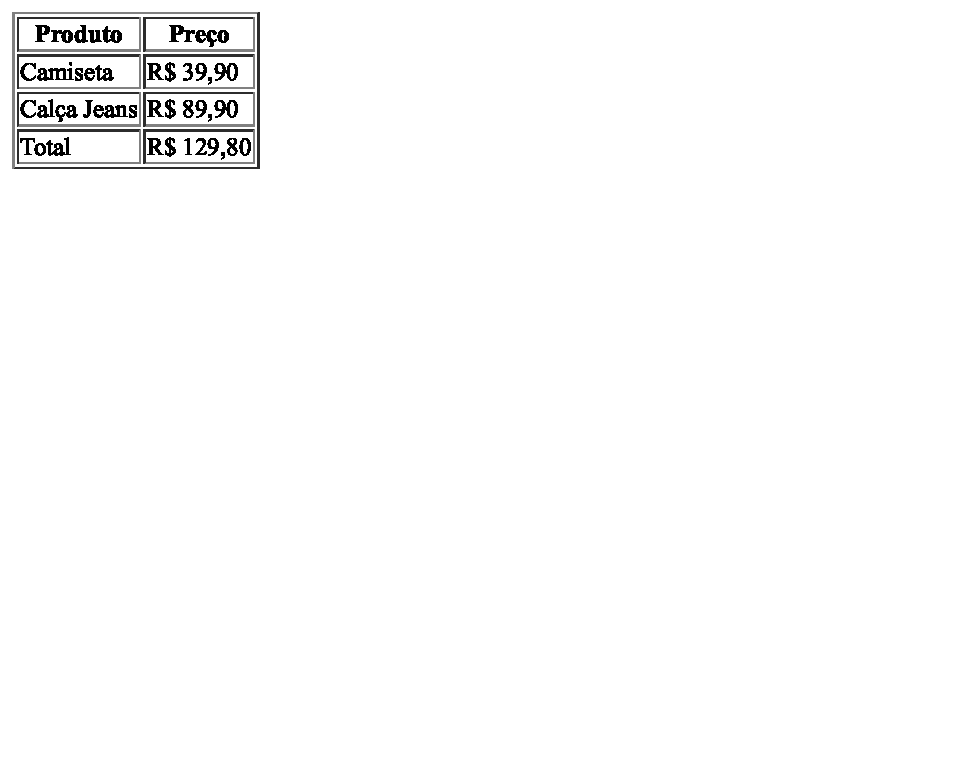
\includegraphics[width=.3\textwidth, trim={0 10cm 12cm 0}]{Images/chapter04/html_table_hbf.pdf}}
    \caption{Renderização da tabela do exemplo \ref{code:table_hbf}.}
    \label{fig:table_hbf}
\end{figure}

\subsection{Mesclagem de Linhas e Colunas}

A mesclagem de linhas e colunas em tabelas HTML é uma técnica que permite combinar várias células em uma única célula, tanto na horizontal quanto na vertical. Isso é feito com os atributos \var{rowspan} (vertical) e \var{colspan} (horizontal) dos elementos \var{<th>} e \var{<td>}. Esses atributos devem ser valorados, respectivamente, com o número de linhas e de colunas que devem ser mescladas, ou seja, com o número de células abaixo ou à direita que devem ter seus espaços tomados pela célula em expansão.

A mesclagem de colunas (\var{colspan}) é usada quando se deseja combinar duas ou mais células adjacentes em uma única célula horizontal. O atributo \var{colspan} é definido na célula que será expandida e indica quantas colunas devem ser ocupadas. Por exemplo, se quisermos expandir uma célula por duas colunas adjacentes, podemos usar o atributo \var{colspan="2"}. O exemplo \ref{code:table_colspan} mostra o código uma tabela HTML com mesclagem de colunas.

\begin{htmlcode}{Tabela com mesclagem de colunas.}{code:table_colspan}
<table border="1">
    <tr>
        <th>Produto</th>
        <th>Preço</th>
        <th colspan="2">Disponibilidade</th>
    </tr>
    <tr>
        <td>Camiseta</td>
        <td>R$ 39,90</td>
        <td>Disponível</td>
        <td>Entrega em 24h</td>
    </tr>
    <tr>
        <td>Calça Jeans</td>
        <td>R$ 89,90</td>
        <td>Indisponível</td>
        <td>-</td>
    </tr>
</table>
\end{htmlcode}

Neste exemplo, a célula que contém a informação de disponibilidade (Disponível ou Indisponível) e a informação de entrega (Entrega em 24h ou -) é mesclada com a célula faltante da coluna à sua direita, utilizando o atributo \var{colspan="2"}. Isso permite que a tabela fique mais organizada e fácil de ler, como mostra a figura \ref{fig:table_colspan}. A quantidade de colunas de uma tabela sempre será igual à quantidade máxima de células em uma linha qualquer. Por conta disso, no caso deste exemplo, a tabela possui 4 colunas, sendo que a última célula da primeira linha ocupa o espaço de duas colunas.

\begin{figure}[ht!]    
    \frame{
    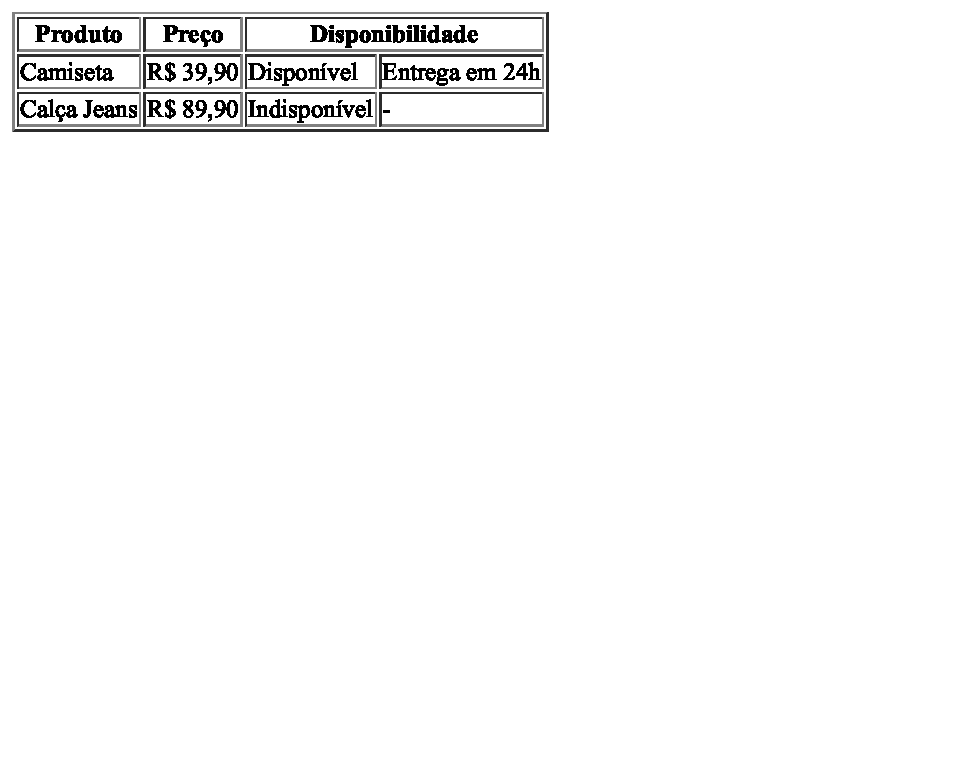
\includegraphics[width=.6\textwidth, trim={0 10.5cm 6.5cm 0}]{Images/chapter04/html_table_colspan.pdf}}
    \caption{Renderização da tabela do exemplo \ref{code:table_colspan}.}
    \label{fig:table_colspan}
\end{figure}

A mesclagem de linhas (\var{rowspan}) é usada quando se deseja combinar duas ou mais células adjacentes em uma única célula vertical. O atributo \var{rowspan} é definido na célula que será mesclada e indica quantas linhas devem ser expandidas. Por exemplo, se quisermos expandir uma célula para que ela ocupe duas linhas adjacentes, podemos usar o atributo \var{rowspan="2"}. O exemplo \ref{code:table_rowspan} mostra o código uma tabela HTML com mesclagem de linhas.

\begin{htmlcode}{Tabela com mesclagem de linhas.}{code:table_rowspan}
<table border="1">
    <tr>
        <th>Produto</th>
        <th>Preço</th>
    </tr>
    <tr>
        <td rowspan="2">Conjunto de Panelas</td>
        <td>R$ 199,90</td>
    </tr>
    <tr>
        <td>R$ 189,90</td>
    </tr>
    <tr>
        <td>Liquidificador</td>
        <td>R$ 99,90</td>
    </tr>
</table>
\end{htmlcode}

Neste exemplo \ref{code:table_rowspan}, a célula que contém o nome do produto (Conjunto de Panelas) é mesclada com a célula da linha abaixo, utilizando o atributo \var{rowspan="2"}. Isso permite que a tabela fique mais compacta e fácil de ler, como mostra a figura \ref{fig:table_rowspan}

\begin{figure}[ht!]    
    \frame{
    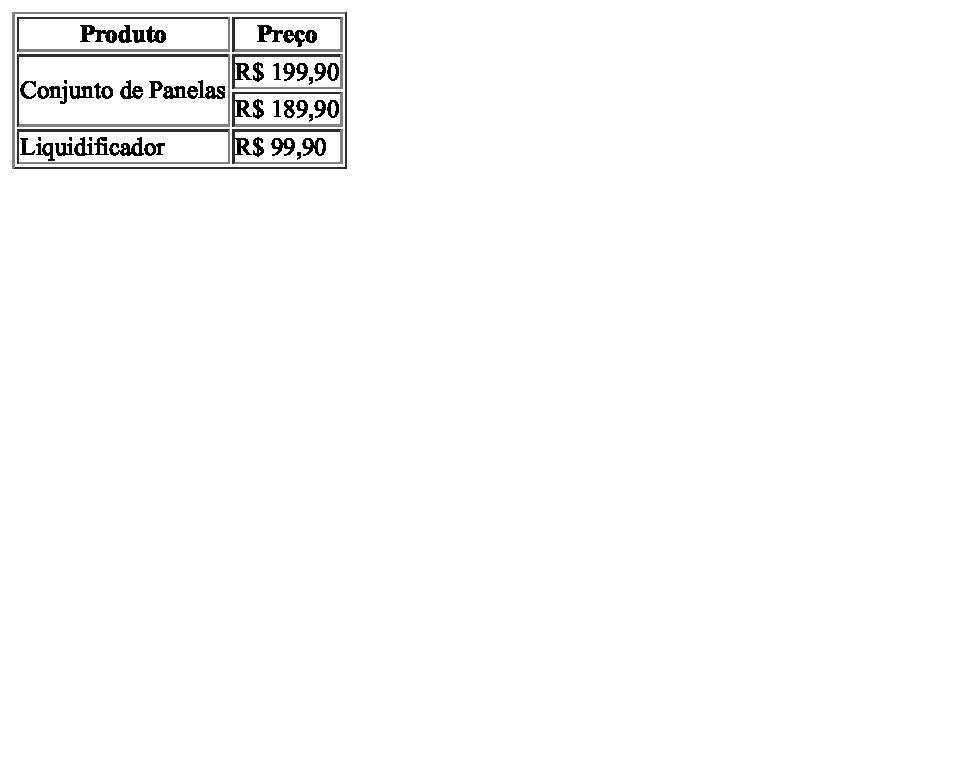
\includegraphics[width=.4\textwidth, trim={0 10cm 10cm 0}]{Images/chapter04/html_table_rowspan.pdf}}
    \caption{Renderização da tabela do exemplo \ref{code:table_rowspan}.}
    \label{fig:table_rowspan}
\end{figure}

A mesclagem de linhas e colunas é uma técnica avançada de criação de tabelas HTML que requer planejamento cuidadoso e atenção aos detalhes. É importante lembrar que a mesclagem de linhas e colunas deve ser usada com moderação e apenas quando necessário, uma vez que pode tornar a tabela mais complexa e difícil de ler. 

Além disso, a mesclagem de linhas e colunas pode afetar a acessibilidade da tabela, tornando-a menos legível para usuários de tecnologias assistivas, como usuários de leitores de tela. Uma boa prática é sempre testar a tabela em diferentes tamanhos de tela e verificar se ela está se comportando corretamente. Além disso, é importante usar os elementos de cabeçalho (\var{<th>}) para identificar os cabeçalhos de coluna e linha, tornando a tabela mais acessível e legível.

Em resumo, a mesclagem de linhas e colunas em tabelas HTML é uma técnica útil e poderosa para criar estruturas de tabela mais complexas. Combinada com outras técnicas de estilização e formatação, as tabelas podem ser uma maneira eficaz de organizar e apresentar informações em formato tabular para os usuários. Para concluir esta seção, o exemplo \ref{code:table_colrowspan} mostra uma tabela com mesclagem de linhas e colunas, conforme ilustra a figura \ref{fig:table_colrowspan}.

\begin{htmlcode}{Tabela com mesclagem de linhas e colunas.}{code:table_colrowspan}
<table border="1">
    <tr>
        <th>Produto</th>
        <th colspan="2">Preço</th>
    </tr>
    <tr>
        <td rowspan="2">Conjunto de Panelas</td>
        <td>À prazo</td>
        <td>R$ 199,90</td>
    </tr>
    <tr>
        <td>À vista</td>
        <td>R$ 189,90</td>
    </tr>
    <tr>
        <td>Liquidificador</td>
        <td>Somente à vista</td>
        <td>R$ 99,90</td>
    </tr>
</table>
\end{htmlcode}

\begin{figure}[ht!]    
    \frame{
    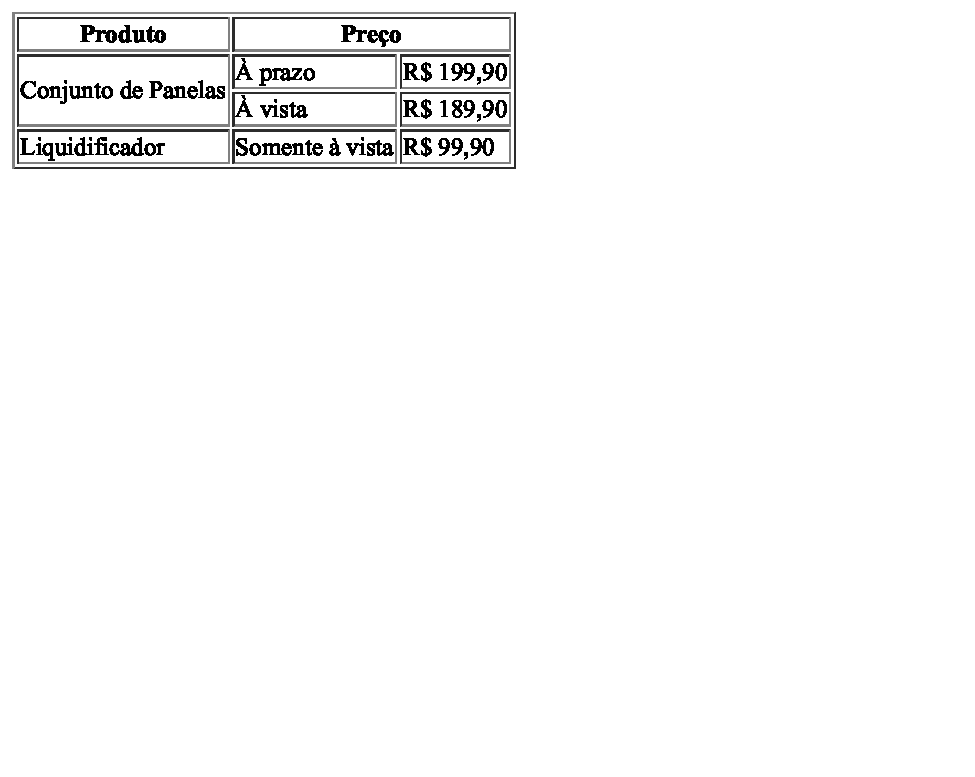
\includegraphics[width=.6\textwidth, trim={0 10cm 7.5cm 0}]{Images/chapter04/html_table_colrowspan.pdf}}
    \caption{Renderização da tabela do exemplo \ref{code:table_colrowspan}.}
    \label{fig:table_colrowspan}
\end{figure}

\section{Exercícios Propostos}

Essa série de exercícios envolve os conceitos abordados neste capítulo e também \textbf{pode demandar alguma pesquisa}. Reserve um tempo e um local adequados para fazer os exercícios sem distrações. Assim você absorverá muito mais o conteúdo estudado. \textbf{Observação}: para os exercícios envolvendo tabelas, use o atributo para inserir borda.

\begin{exercise}
Crie uma lista de compras de supermercado com pelo menos 5 itens.
\end{exercise}

\begin{exercise}
Crie uma lista de características de um produto ou serviço oferecido por uma loja virtual qualquer.
\end{exercise}

\begin{exercise}
Crie uma lista de redes sociais em que uma pessoa ou empresa pode estar presente.
\end{exercise}

\begin{exercise}
Crie uma lista numerada de passos para realizar uma receita de bolo de chocolate.
\end{exercise}

\begin{exercise}
Crie uma lista de rankings ou classificações como os melhores filmes que você já assistiu.
\end{exercise}

\begin{exercise}
Crie uma lista ordenada de tarefas que você executa do momento em que acorda até o momento em que deita para dormir.
\end{exercise}

\begin{exercise}
Crie uma lista com 5 termos e suas definições para um glossário de redes sociais.
\end{exercise}

\begin{exercise}
Crie uma lista com 5 adjetivos em inglês e suas respectivas traduções para português.
\end{exercise}

\begin{exercise}
Crie uma lista de sinônimos e antônimos para 5 palavras-chave de um dicionário.
\end{exercise}

\begin{exercise}
Crie uma lista de abreviações e seus significados sobre astronomia.
\end{exercise}

\begin{exercise}
Crie uma tabela que exiba uma lista de 5 preços de produtos. Inclua uma coluna para o nome do produto, outra para o preço e uma terceira para uma breve descrição do produto.
\end{exercise}

\begin{exercise}
Crie uma tabela que exiba uma programação de 5 eventos para uma conferência. Inclua colunas para o nome do evento, o horário, a localização e a descrição.
\end{exercise}

\begin{exercise}
Crie uma tabela com três colunas e três linhas, e mescle a primeira célula das três linhas para criar uma célula que ocupe duas colunas. Adicione conteúdo a cada célula para exibir informações sobre um produto.
\end{exercise}

\begin{exercise}
Crie uma tabela que exiba informações de contato para uma empresa. Inclua colunas para o nome, o endereço, o telefone e o e-mail, sendo que o telefone e o e-mail devem estar sob o mesmo título (Contatos).
\end{exercise}

\begin{exercise}
Crie uma tabela que exiba informações sobre um time de futebol. Inclua colunas para o nome do jogador e para alguns dados técnicos, incluindo a posição, o número da camisa e as estatísticas de desempenho, sendo que essas 3 últimas informações devem ficar em 3 linhas diferentes, enquanto a coluna com o nome do jogador deve se expandir por essas 3 linhas.
\end{exercise}

\begin{exercise}
Crie uma tabela que exiba uma lista de 3 tarefas com datas de início e de conclusão. Mescle as 2 primeiras células da primeira linha para criar uma célula que ocupe 2 colunas, e mescle as 3 primeiras células da primeira coluna para criar uma célula que ocupe 3 linhas. Em síntese, a primeira célula da tabela vai ocupar 2 linhas e 3 colunas e deve ter o título ``Tarefas'', enquanto as demais células devem armazenar as demais informações, ou seja, o título da tarefa, a data de início e a data de conclusão.
\end{exercise}

\begin{exercise}
Crie uma tabela que exiba informações sobre o desempenho de 3 atletas em diferentes eventos esportivos A, B e C. O primeiro atleta participou dos eventos A e B, o segundo participou de B e C, e o terceiro participou de A, B e C. A tabela deve ter 3 colunas. A primeira deve ter o nome do atleta expandido para a quantidade de linhas correspondente à quantidade de eventos que ele participou. A segunda coluna deve apresentar em linhas distintas os eventos que o atleta participou e a terceira coluna deve mostrar o tempo do atleta no respectivo evento.
\end{exercise}

\begin{exercise}
Faça uma tabela idêntica à apresentada abaixo. \\
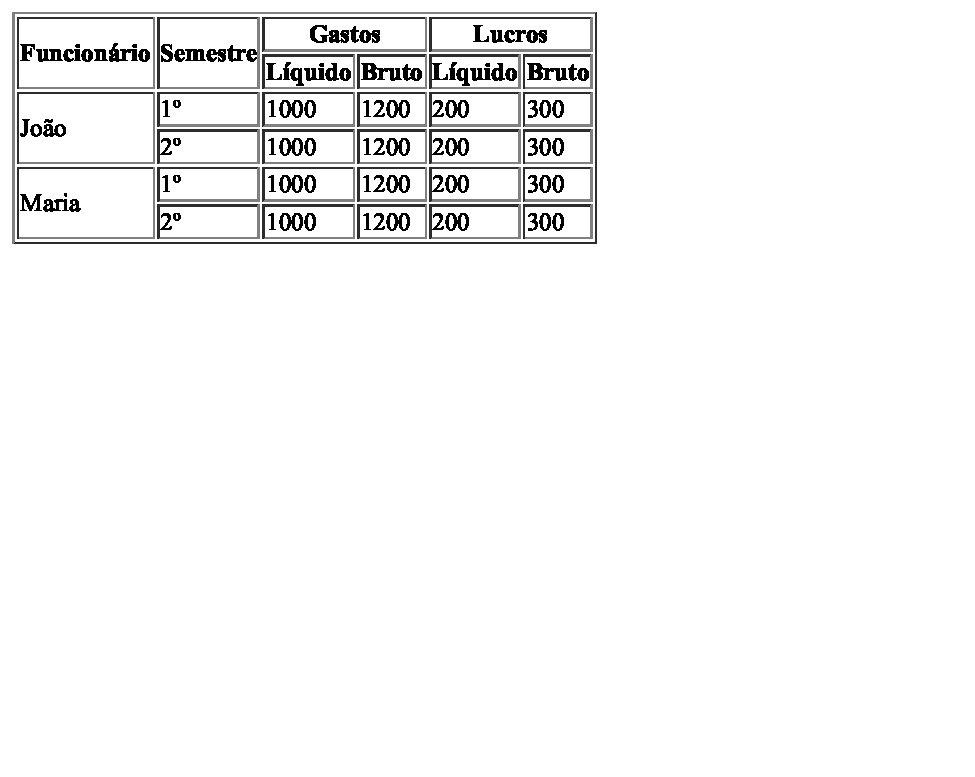
\includegraphics[width=.5\textwidth, trim={0 8.8cm 7cm 0}]{Images/chapter04/html_ex_table_01.pdf}     
\end{exercise}

\begin{exercise}
Faça uma tabela idêntica à apresentada abaixo. \\
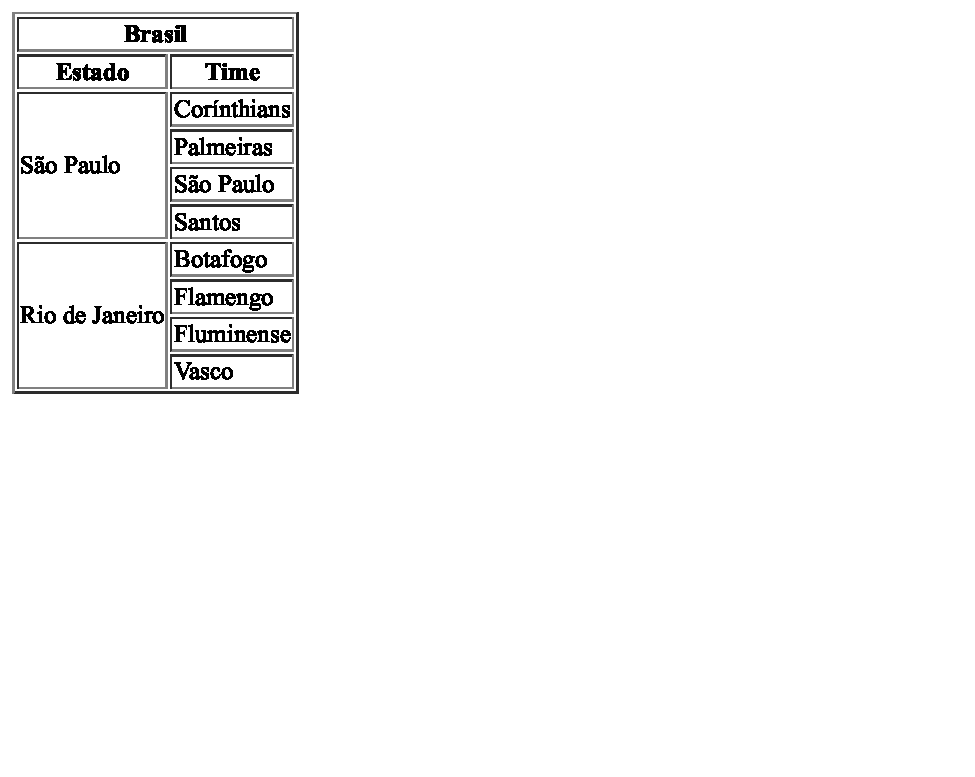
\includegraphics[width=.5\textwidth, trim={0 6.3cm 7cm 0}]{Images/chapter04/html_ex_table_02.pdf}     
\end{exercise}

\begin{exercise}
Faça uma tabela idêntica à apresentada abaixo. \\
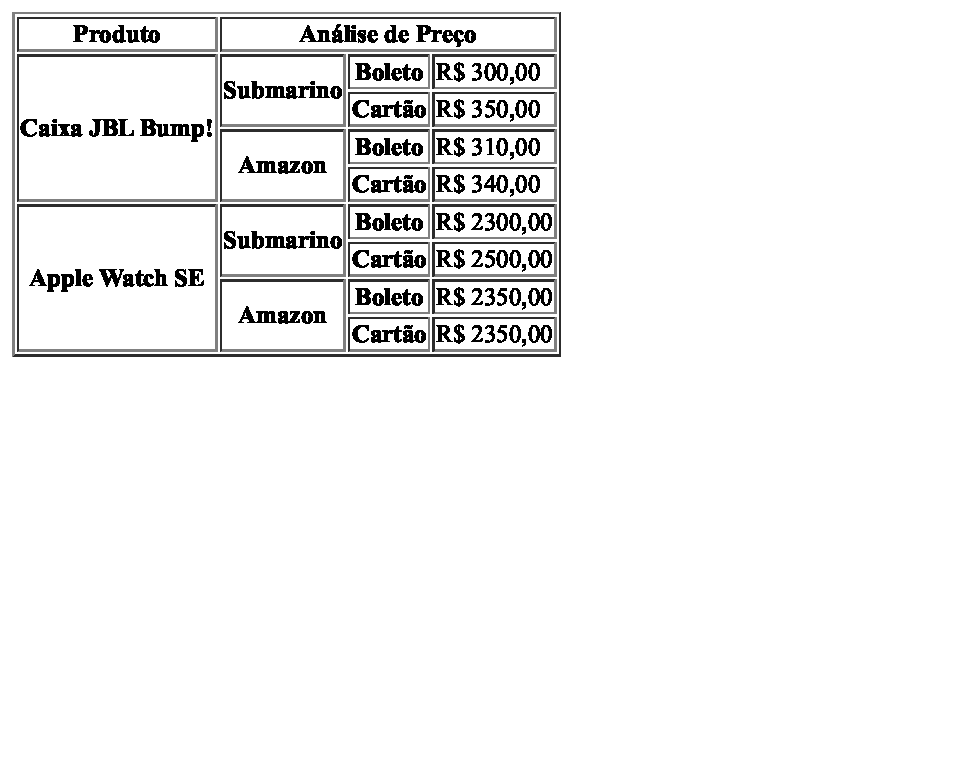
\includegraphics[width=.5\textwidth, trim={0 6.85cm 7cm 0}]{Images/chapter04/html_ex_table_03.pdf}     
\end{exercise}

\section{Considerações Sobre o Capítulo}

Este capítulo apresentou como criar listas e tabelas em HTML. Vimos as listas não ordenadas, ordenadas e de definições, bem como tabelas simples, com agrupamento de cabeçalho, conteúdo e rodapé e com linhas e colunas mescladas. No capítulo seguinte veremos como apresentar imagens em um documento HTML.